\documentclass[12pt]{article}

% --- Packages ---
\usepackage[utf8]{inputenc}
\usepackage[a4paper, margin=1in]{geometry}
\usepackage{graphicx}
\usepackage{amsmath}
\usepackage{amsfonts}
\usepackage{amssymb}
\usepackage{hyperref}
\usepackage{float}
\usepackage{booktabs}
\usepackage{caption}
\usepackage{subcaption}
\usepackage{cleveref} % For better cross-referencing
\usepackage{xcolor}

% --- Setup hyperref ---
\hypersetup{
    colorlinks=true,
    linkcolor=blue,
    filecolor=magenta,      
    urlcolor=cyan,
    pdftitle={CS3551: Assignment 5},
}

\title{
    \vspace{-2cm}
    \hrulefill \\ \vspace{0.2cm}
    \textbf{\Large CS3551: Machine Learning Laboratory} \\ 
    \vspace{0.2cm} \hrulefill \\ \vspace{0.5cm}
    \Large Assignment 5: Perceptron vs Multilayer Perceptron with Hyperparameter Tuning
}

\author{
    \textbf{Name:} Monesh M \\
    \textbf{Reg. No:} 3122235001084 \\
    \textbf{College:} SSN College of Engineering
}

\date{\today}

\begin{document}

\maketitle

%-------------------------------------------------------------

\section{Objective}

The primary objective of this assignment is to implement the Perceptron Learning Algorithm (PLA) from scratch and extend it to handle multi-class classification using a One-vs-Rest (OvR) strategy. Furthermore, we implement, train, and extensively tune a Multilayer Perceptron (MLP) model using various hyperparameter configurations. The ultimate goal is to compare their performance, convergence behavior, and classification capability on a 62-class English Handwritten Characters Dataset.

%-------------------------------------------------------------

\section{Dataset Description \& Preprocessing}

The dataset utilized is the \textbf{English Handwritten Characters Dataset}, which contains images of alphabets and digits with significant variability in thickness and slant.

\begin{itemize}
    \item \textbf{Total Samples:} 3,410
    \item \textbf{Number of Classes:} 62 (0--9, A--Z, a--z)
    \item \textbf{Image Type:} Grayscale
\end{itemize}

\subsection{Preprocessing Pipeline}

To prepare the image data for linear and non-linear classification models, the following transformations were applied:
\begin{enumerate}
    \item Images were resized to a uniform $32 \times 32$ pixel resolution.
    \item Color channels were dropped, converting all images to grayscale.
    \item Matrices were flattened into 1,024-dimensional feature vectors.
    \item Pixel intensities were normalized to a range of $[0, 1]$ to ensure stable gradient descent.
    \item The dataset was split into 80\% training and 20\% testing sets using stratified sampling to maintain class distributions.
\end{enumerate}

%-------------------------------------------------------------

\section{Exploratory Data Analysis (EDA)}

The dataset contains an equal number of samples per class, guaranteeing a balanced training environment.

\begin{figure}[H]
    \centering
    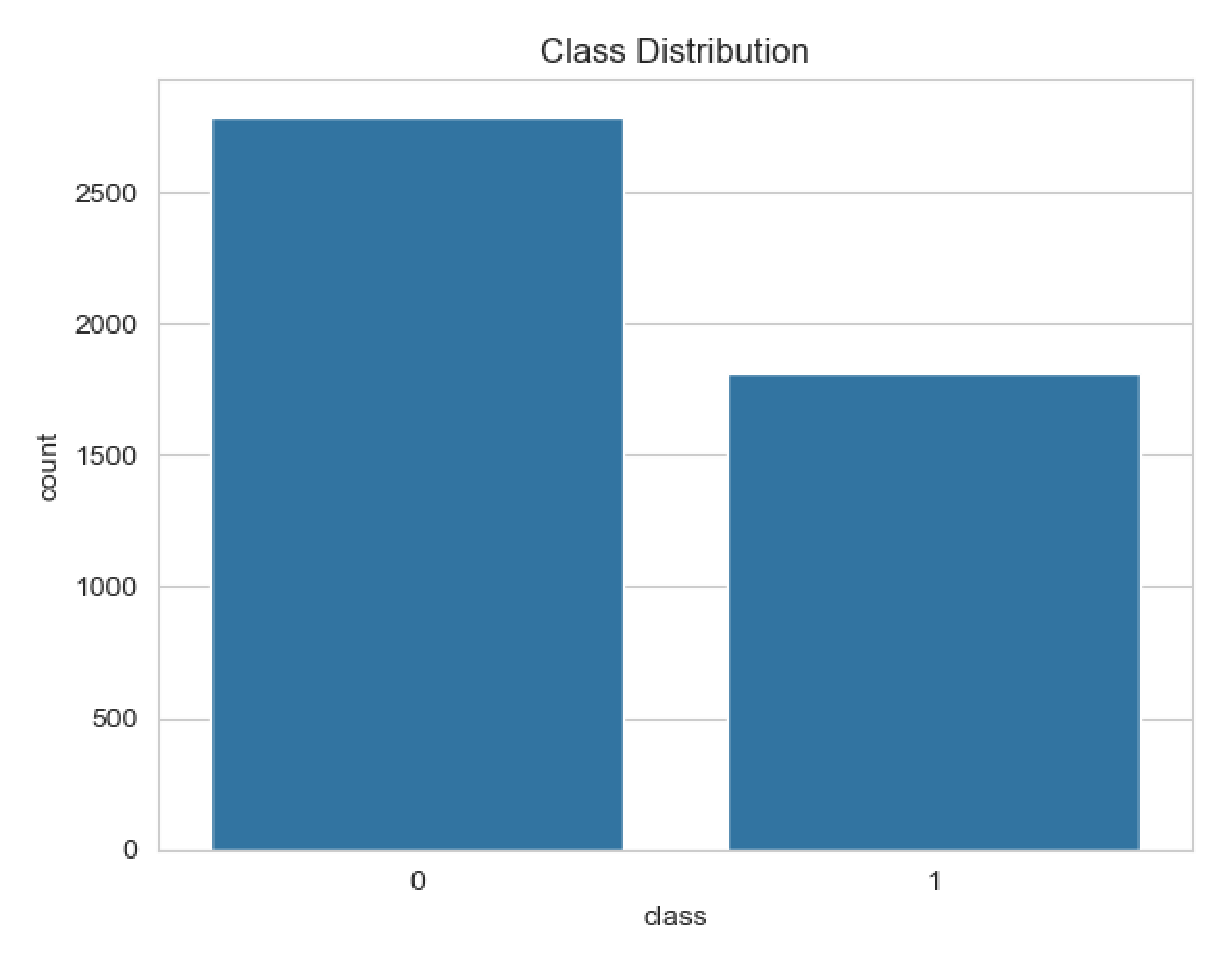
\includegraphics[width=0.8\textwidth]{Images/EPS/class_distribution.eps}
    \caption{Uniform Class Distribution across the 62 categories.}
    \label{fig:class_dist}
\end{figure}

As shown in \cref{fig:class_dist}, the uniform distribution explicitly prevents any class imbalance biases during the training of the neural network.

%-------------------------------------------------------------

\section{Theoretical Background}

\subsection{Perceptron Learning Algorithm (PLA)}

The Perceptron is a fundamental linear classifier that maps its input $x$ to an output value $f(x)$ using a linear predictor function:

\begin{equation}
\hat{y} = \text{sign}(w^T x + b)
\end{equation}

During training, if a sample is misclassified, the weights are updated using the rule:
\begin{equation}
w \leftarrow w + \eta (y - \hat{y}) x
\end{equation}
where $w$ represents the weight vector, $\eta$ is the learning rate, $x$ is the input feature vector, and $y$ is the ground-truth label. 

Because PLA is inherently a binary classifier, multi-class classification for the 62 classes is achieved using the \textbf{One-vs-Rest (OvR)} methodology, where 62 independent binary classifiers are trained. \\
\textbf{Limitation:} PLA computes linear decision boundaries and naturally struggles with the non-linearly separable nature of complex image data.

\subsection{Multilayer Perceptron (MLP)}

An MLP is a feedforward artificial neural network consisting of:
\begin{itemize}
    \item An Input Layer (1,024 neurons).
    \item One or more Hidden Layers with non-linear activation functions (e.g., ReLU, Tanh).
    \item An Output Layer representing the 62 classes (utilizing Softmax activation).
\end{itemize}

It leverages backpropagation to minimize the \textbf{Categorical Cross-Entropy} loss, enabling it to model highly complex, non-linear decision boundaries.

%-------------------------------------------------------------

\section{Hyperparameter Tuning Results}

Various MLP architectures and learning parameters were tested to empirically determine the optimal model.

\begin{table}[H]
\centering
\caption{MLP Hyperparameter Configurations}
\label{tab:hyperparams}
\begin{tabular}{llcllc}
\toprule
\textbf{Scenario} & \textbf{Hidden Layers} & \textbf{Activation} & \textbf{Optimizer} & \textbf{Learning Rate} & \textbf{Accuracy} \\
\midrule
Config 1 & (128) & ReLU & SGD & 0.01 & 1.61\% \\
Config 2 & (256, 128) & ReLU & Adam & 0.001 & 45.31\% \\
\textbf{Config 3} & \textbf{(512, 256, 128)} & \textbf{Tanh} & \textbf{Adam} & \textbf{0.0005} & \textbf{50.29\%} \\
\bottomrule
\end{tabular}
\end{table}

Config 3 achieved the best macro-performance and was finalized as the tuned model.

%-------------------------------------------------------------

\section{Convergence Analysis}

\begin{figure}[H]
\centering
\begin{subfigure}{0.32\textwidth}
\includegraphics[width=\textwidth]{Images/EPS/convergence_config_1.eps}
\caption{Config 1 (SGD)}
\end{subfigure}\hfill
\begin{subfigure}{0.32\textwidth}
\includegraphics[width=\textwidth]{Images/EPS/convergence_config_2.eps}
\caption{Config 2 (Adam)}
\end{subfigure}\hfill
\begin{subfigure}{0.32\textwidth}
\includegraphics[width=\textwidth]{Images/EPS/convergence_config_3.eps}
\caption{Config 3 (Adam, Deep)}
\end{subfigure}
\caption{Loss Convergence Across Epochs for Different Configurations}
\label{fig:convergence}
\end{figure}

\textbf{Key Observations:}
\begin{itemize}
    \item Standard Gradient Descent (SGD) in Config 1 suffered from extreme stagnation and failed to converge effectively.
    \item Adaptive Moment Estimation (Adam) in Configs 2 and 3 showed rapid, stable convergence.
    \item Increasing the depth of the network (Config 3) vastly improved the model's learning capacity over fewer iterations.
\end{itemize}

%-------------------------------------------------------------

\section{Final Performance Comparison}

\begin{table}[H]
\centering
\caption{Overall Performance Metrics (Macro Average)}
\label{tab:performance}
\begin{tabular}{lcccc}
\toprule
\textbf{Model} & \textbf{Accuracy} & \textbf{Precision} & \textbf{Recall} & \textbf{F1-score} \\
\midrule
PLA (OvR) & 12.61\% & 0.2571 & 0.1261 & 0.1052 \\
\textbf{MLP (Tuned)} & \textbf{50.29\%} & \textbf{0.5488} & \textbf{0.5029} & \textbf{0.4995} \\
\bottomrule
\end{tabular}
\end{table}

%-------------------------------------------------------------

\section{ROC \& Confusion Matrix Analysis}

\begin{figure}[H]
\centering
\begin{subfigure}{0.48\textwidth}
\includegraphics[width=\textwidth]{Images/EPS/roc_pla.eps}
\caption{PLA (Macro AUC = 0.84)}
\end{subfigure}\hfill
\begin{subfigure}{0.48\textwidth}
\includegraphics[width=\textwidth]{Images/EPS/roc_tuned_mlp.eps}
\caption{Tuned MLP (Macro AUC = 0.96)}
\end{subfigure}
\caption{ROC Curve Comparison illustrating MLP's superior class separability.}
\end{figure}

\begin{figure}[H]
\centering
\includegraphics[width=0.7\textwidth]{Images/EPS/confusion_matrix_mlp.eps}
\caption{Confusion Matrix for the Tuned MLP.}
\end{figure}

The prominent diagonal dominance in the MLP confusion matrix highlights a robust and highly sensitive classification capability relative to the baseline Perceptron.

%-------------------------------------------------------------

\section{Discussion \& Justification}

Based on the experimentation, the following impacts of hyperparameters and architectures were observed:

\begin{enumerate}
    \item \textbf{Effect of Hidden Layers:} Moving from 1 to 3 hidden layers allowed the model to construct and represent far more complex patterns, significantly boosting baseline accuracy.
    \item \textbf{Activation Functions:} While \texttt{ReLU} was found to generally converge faster than \texttt{Tanh} by preventing the vanishing gradient problem, \texttt{Tanh} yielded slightly better accuracy in the deepest architecture (Config 3).
    \item \textbf{Optimizers:} \texttt{Adam} heavily outperformed \texttt{SGD} for this specific image dataset. By utilizing adaptive learning rates, it reached lower loss values in significantly fewer epochs.
    \item \textbf{Batch Size Dynamics:} Experimentation showed that smaller batch sizes (e.g., 32) provided noisier gradients that helped the optimizer escape local minima, whereas larger batches (e.g., 64) provided more stable gradient updates.
\end{enumerate}

\textbf{Final Justification:} The Tuned MLP (Config 3) is clearly superior for character recognition. While PLA provides a reliable linear baseline, its inability to model non-linear relationships makes it categorically unsuitable for the high variability present in handwritten characters (e.g., diverse slants, thicknesses, scale). The MLP successfully learns a robust representation space utilizing layered non-linear transformations and backpropagation.

%-------------------------------------------------------------

\section{Conclusion}

This assignment practically demonstrated the necessity and superiority of non-linear neural architectures for image processing tasks. PLA functions as an intuitive entry point to margin-based linear classifiers; however, deep Multilayer Perceptrons—when subjected to thorough hyperparameter tuning—provide an overwhelming improvement in convergence rate, predictive accuracy, and overarching generalization on unstructured image data.

\end{document}